\documentclass[a4paper]{article}
% -------------------------------PACKAGES-------------------------------
\usepackage{amsmath,amsfonts,amssymb}   % for math
\usepackage{indentfirst}    % for indenting first para after section
\usepackage{xcolor}         % for coloured text
\usepackage{listings}       % for Python text
\usepackage{graphicx}       % for images
\usepackage{hyperref}       % for hyperlinks & internal references
\usepackage[utf8]{inputenc} % for best practice
\setlength{\parskip}{1em}   % length between paras

% Python-style environment setup
\definecolor{codegreen}{rgb}{0,0.6,0}
\definecolor{codegray}{rgb}{0.5,0.5,0.5}
\definecolor{codepurple}{rgb}{0.58,0,0.82}
\definecolor{backcolour}{rgb}{0.95,0.95,0.92}

\lstdefinestyle{mystyle}{
    backgroundcolor=\color{backcolour},   
    commentstyle=\color{codegreen},
    keywordstyle=\color{magenta},
    numberstyle=\tiny\color{codegray},
    stringstyle=\color{codepurple},
    basicstyle=\ttfamily\footnotesize,
    breakatwhitespace=false,         
    breaklines=true,                 
    captionpos=b,                    
    keepspaces=true,                 
    numbers=left,                    
    numbersep=5pt,                  
    showspaces=false,                
    showstringspaces=false,
    showtabs=false,                  
    tabsize=2
}
\lstset{style=mystyle}

% Boilerplate
\title{CAB203 Project Report\vspace{-3ex}}
\author{Johnny Madigan}
\date{\vspace{-3ex}June 2021\vspace{20ex}}

\begin{document}
\maketitle
\begin{center}
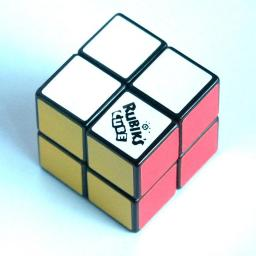
\includegraphics[width=4cm]{rubik.jpg}
\end{center}
\newpage
\tableofcontents
\newpage

% ---------------------INTRODUCTION---------------------
\section{Introduction}\label{sec:introduction}
\par Since the beginning of mankind we have been enthralled by puzzles, because of the challenges they pose and our desire to solve things. Fast-forward to now, and some puzzles have become infamous through their complexity and deceiving looks. One such puzzle is the Pocket Cube, smaller cousin to the iconic Rubik’s Cube.

\par The challenge comes from twisting and turning the cube until each face is one colour. From its fame, the internet has been flooded with algorithms so that anyone can solve the cube themselves. Unfortunately, these algorithms are designed to solve the cube in the least amount of time, not the least amount of moves.

\par This is where our puzzle comes in. No matter what scrambled Pocket Cube we are given, we must figure out the smallest number of moves required to solve it. We will define moves as quarter turns only.

% ---------------------INSTANCE MODEL---------------------
\section{Instance model}\label{sec:instance}
\subsection{Encoding the cube}
\par Using the Python language, we will encode cubes as a single string. The string will comprise of 24 characters, which will reflect the 24 stickers on a Pocket Cube. The diagram helps visualise how a Pocket Cube translates into our encoded instance. An instance that we can easily manipulate and always kept as one argument.

\begin{center}
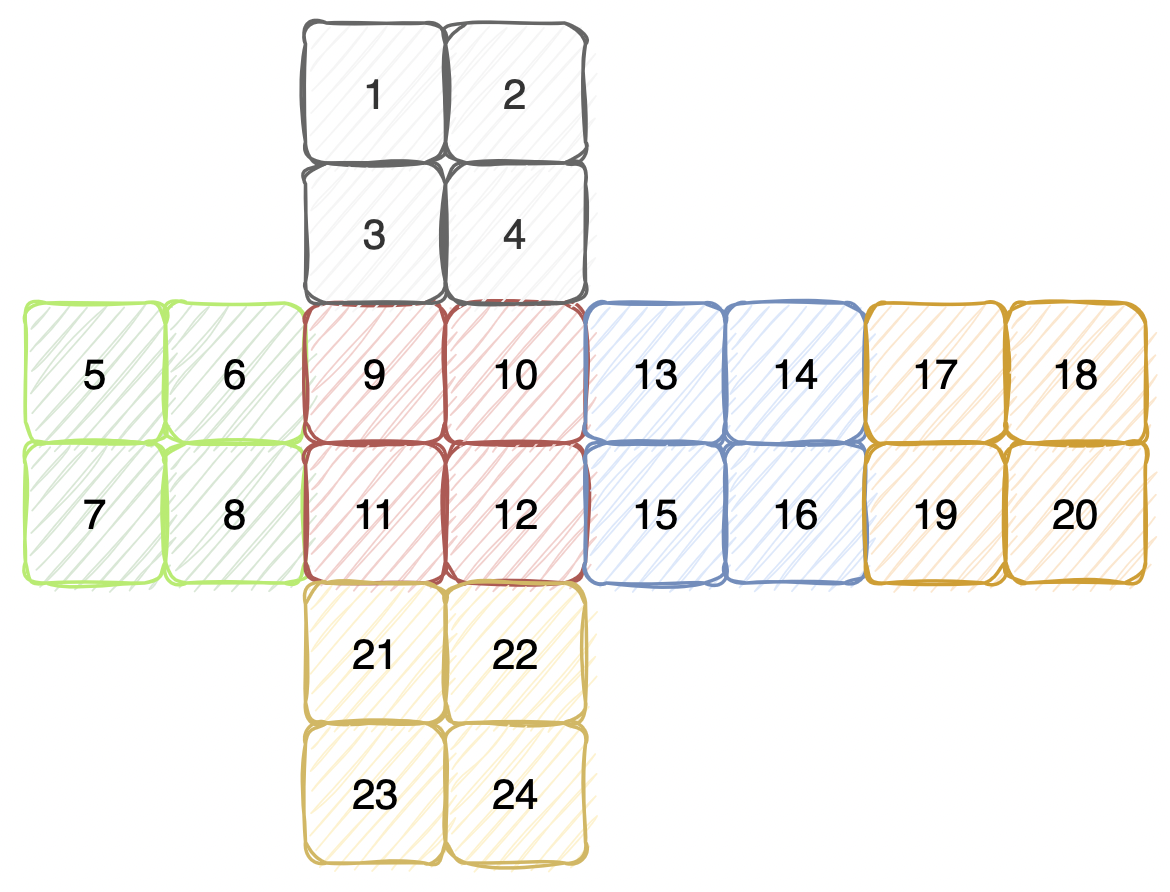
\includegraphics[width=5.9cm]{encoded.png}
\end{center}

\newpage

\par After unravelling any real-life Pocket Cube like the diagram above, we can follow the order of the numbers and note the sticker’s colour to encode the cube into our instance model. E.g, the instance will look like this using the following characters to represent the colours:

\begin{center}
\colorbox{black}{\textcolor{white}{W}}
\textcolor{red}{R}
\textcolor{yellow}{Y}
\textcolor{green}{G}
\textcolor{blue}{B}
\textcolor{orange}{O}
\end{center}

\begin{lstlisting}[language=Python]
instance = "WWWWGGGGRRRRBBBBOOOOYYYY" # a solved cube
\end{lstlisting}

\subsection{Achieving all permutations}
\label{permutations}

\par Research shows us that a Pocket Cube has 3,674,160 possible permutations (“Pocket Cube”, n.d.). Given this, we can validate the instance if it can be transform into over 3.6 million permutations. Briefly breaking down how this number was found; we start with 8 cubies (corner pieces), each of which can be in 8 possible positions.

\[8!\]

\par Furthermore, each cubie can be independently rotated. With 3 exposed stickers, this gives us an additional 3 permutations per cubie. However, one of the cubie's orientation is fixed as it is the pivot point for rotating our cube. Which means only seven cubies will have 3 possible orientations.

\[8!*3^7\]

\par Finally, we do not care about the orientation of the cube in 3D space.

\[\frac{8!*3^7}{24} = 3,674,160\]

\par With the instance comprising of 24 characters, it is possible to generate up to 6.204484e+23 permutations, proving its capability. After defining the six legal quarter turns following the math above, the permutations are reduced to 3,674,160. Each of the moves below will rearrange the position of the characters in the string (0-based index). Groups of three characters will be rearranged to simulate a corner piece changing position/orientation, with one being fixed and never touched (chars at positions 2,5,17).

\subsection{The six legal quarter turns}

\begin{center}
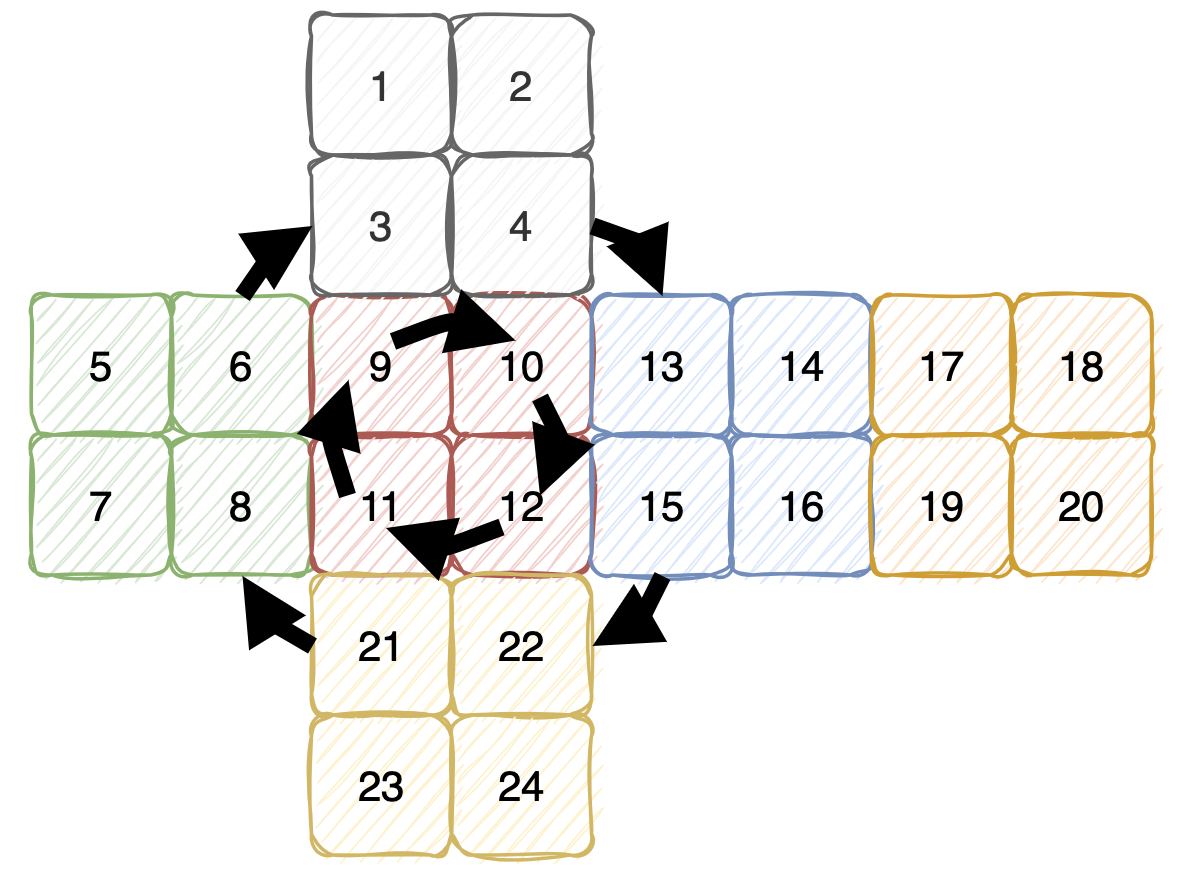
\includegraphics[width=5.9cm]{upface-clockwise.png}\\
\emph{Rotating the ‘UP FACE’ clockwise (U) \& anti-clockwise (U')}
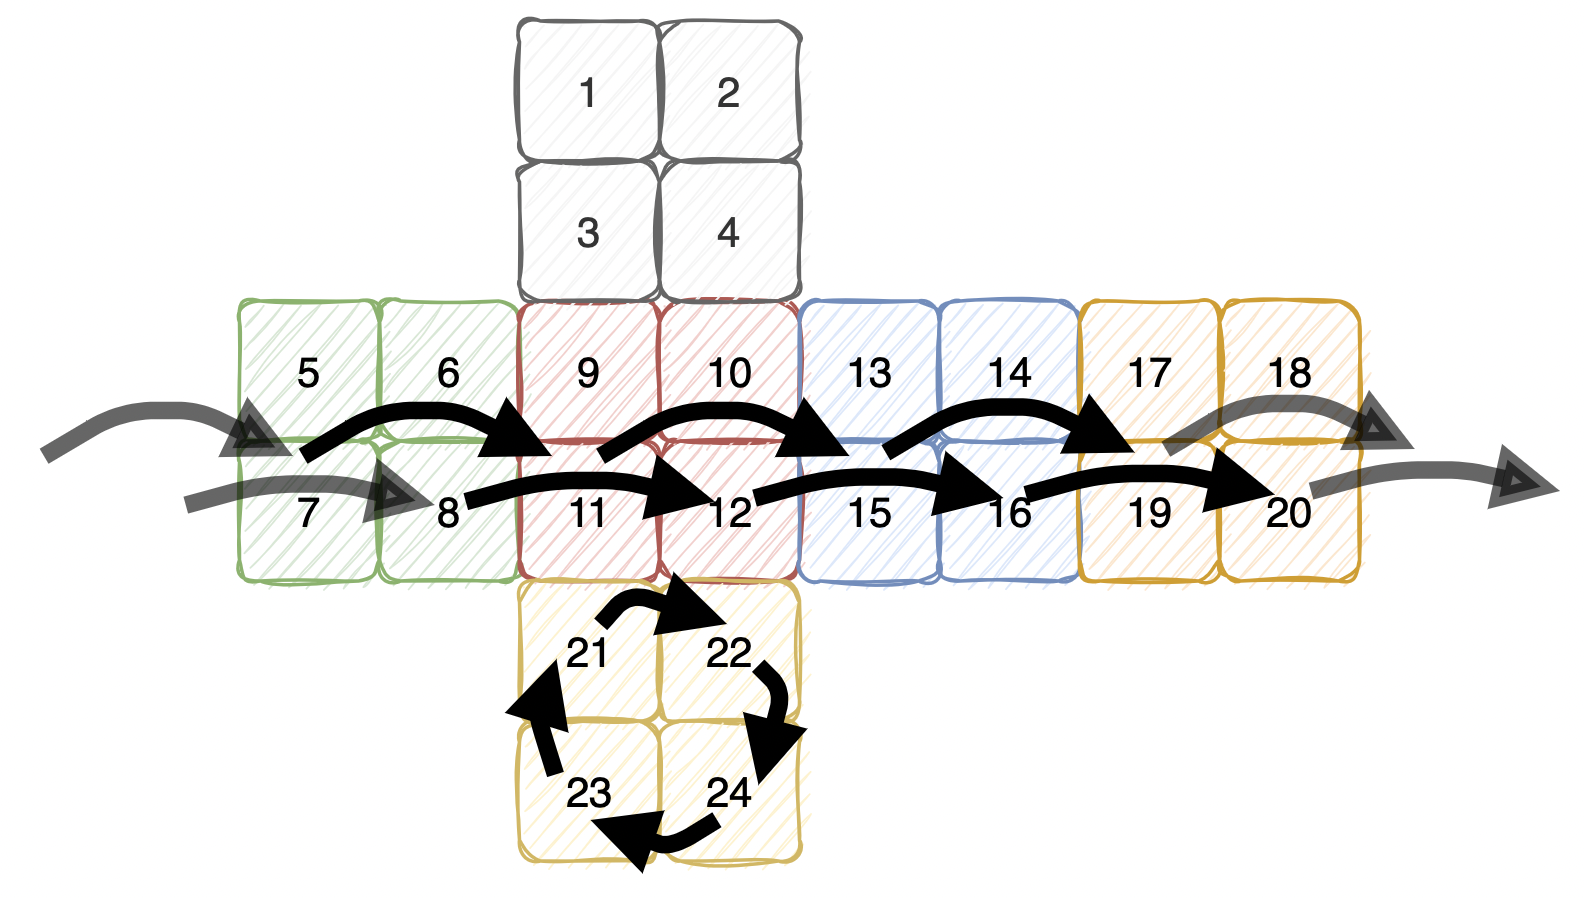
\includegraphics[width=7.2cm]{frontface-clockwise.png}\\
\emph{Rotating the ‘FRONT FACE’ clockwise (F) \& anti-clockwise (F')}
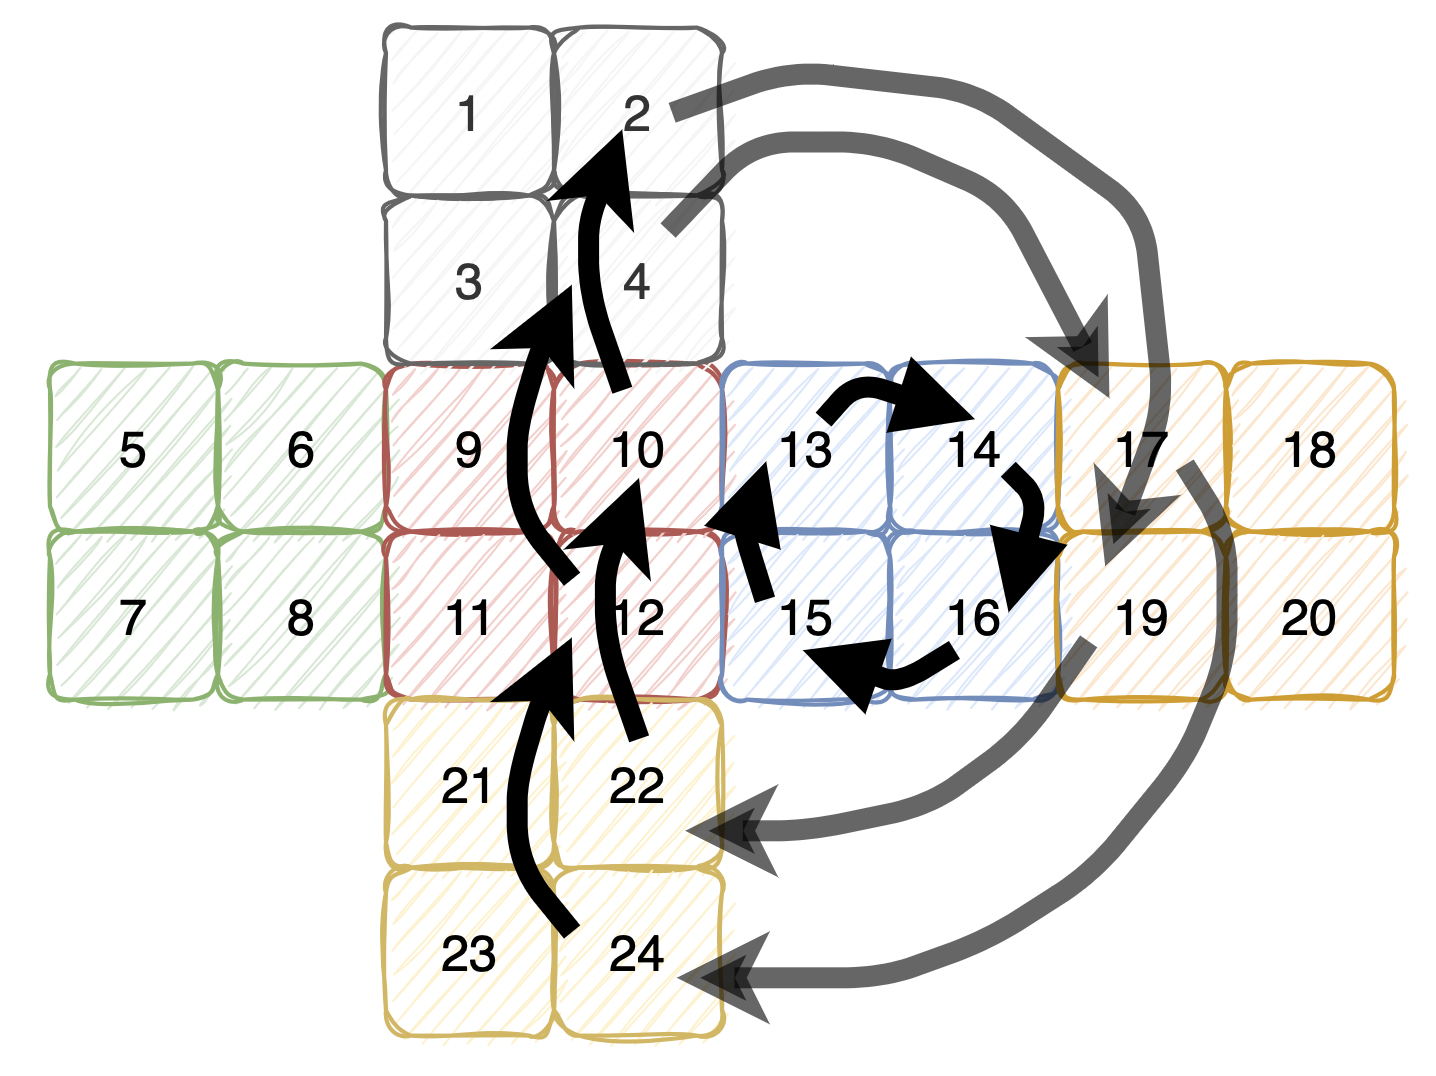
\includegraphics[width=5.9cm]{rightface-clockwise.png}\\
\emph{Rotating the ‘RIGHT FACE’ clockwise (R) \& anti-clockwise (R')}
\end{center}

% ---------------------GRAPH THEORY MODEL---------------------
\section{Graph Theory model}
\subsection{The graph}
\label{graph}

\par Tripi (2017) defines \emph{Cayley Graphs} as a method to ‘\emph{geometrically display the actions of a group}’ and in its true form, a Pocket Cube is just a group of permutations connected through actions (p. 1). The vertices in our \emph{Cayley Graph} are permutations, connected via edges (parent \& derived cubes). New vertices and edges are generated using the generator set (the six legal moves).

\par With the solved cube as the root vertex, the program will start generating the \emph{Cayley Graph} where each vertex will have six children/neighbours/adjacent vertices and the cycle continues. The graph will immediately stop generating once the instance is found, leaving us with a graph to analyse. The diagram below shows a small version of the graph, which will quickly grow up to a diameter of 14. This diameter is known is due to the fact that all Pocket Cubes are solvable within 14 quarter turns or less, assuming the cube was scrambled legally (Garoni et al., 2020).

\begin{center}
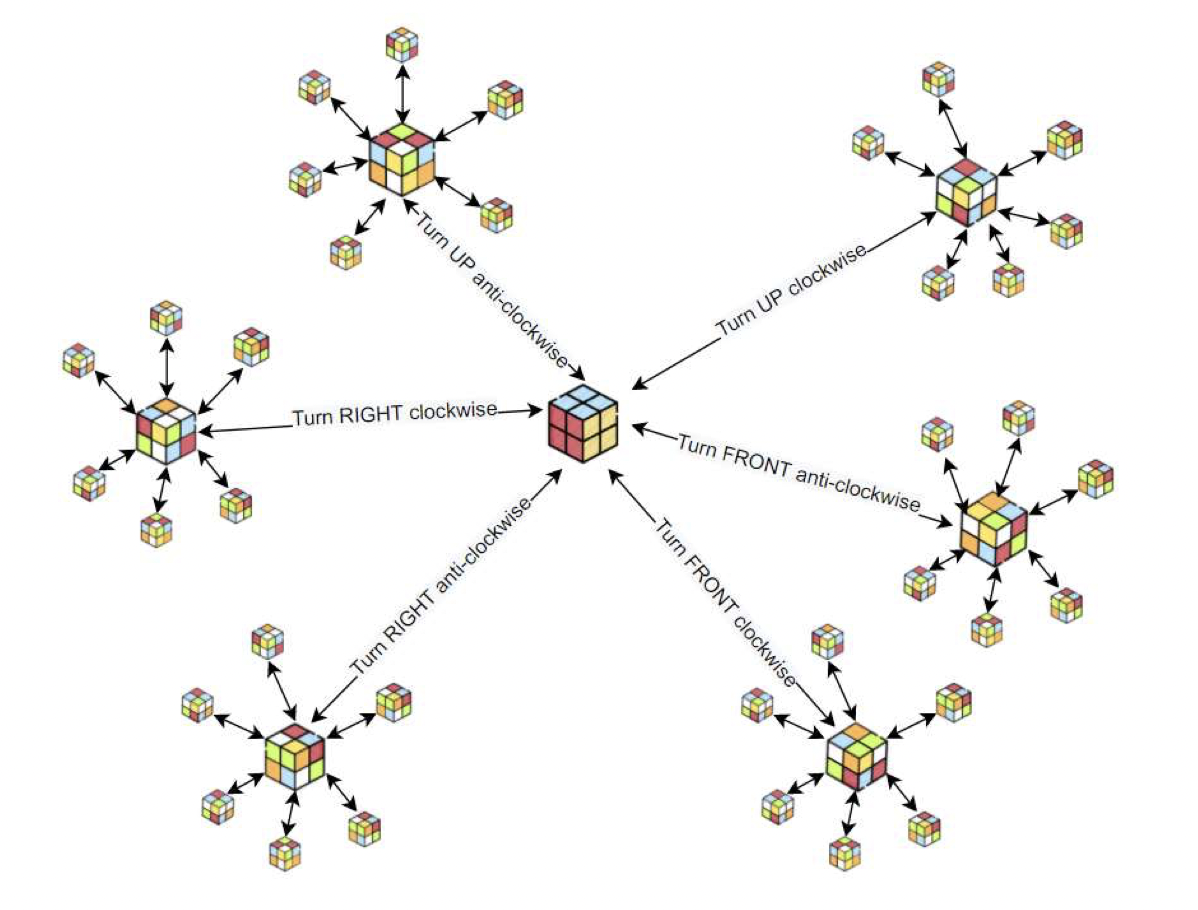
\includegraphics[width=11cm]{cayley.png}\\
\emph{The partial Cayley Graph with the solved cube as the root}
\end{center}

\subsection{Mathematical notation}

\par The group will be set $G$, which will contain subsets of vertices \& edges:

\[G=\{V,E\}\]

\par The generator will be set $S$, which will contain the six quarter turns:

\[S=\{U,U',F,F',R,R'\}\]

\newpage

\par $v$\textsubscript{0} is the solved cube \& the root vertex:

\[v_0\]

\par Generating new vertices will be defined as:

\[v_m = (v_n * s : s\in S, v_n\in V)\]

\par After a new vertex ($v$\textsubscript{$m$}) is generated, it is added to set $V$ if not already a member as sets have unique elements/no duplicates:

\[V\cup \{v_m\}\]

\par After a new vertex ($v$\textsubscript{$m$}) is generated, 2 edges going in each direction will be added to set $E$. This is to keep the graph undirected as derived cubes can always become their parents through a reverse move:

\[E\cup \{(v_m,v_n),(v_n,v_m)\}\]

% ---------------------SOLUTION METHOD---------------------
\section{Solution method}
\par To begin, we must first eliminate all confusion with the instance's orientation as mentioned in Chapter 2, \textbf{\autoref{permutations}}. This is because a no matter how we place the cube on the table, it will always be the same permutation. To deal with this variable, we will generate all 24 possible orientations of the instance and store them in a set. Therefore, the \emph{Cayley Graph} will continue generating while the set of 24 instance orientations does \textbf{not} intersect the group $G$. 

\par The \emph{Cayley Graph} defined in Chapter 3, \textbf{\autoref{graph}} will begin a generating loop starting from the solved cube $v\textsubscript{0}$.

\par For every cube in the current distance class $D\textsubscript{n}$, six new permutations will be made using six algorithms (the legal quarter turns). These algorithms (generator set $S$) will each build a new string a.k.a permutation. These new cubes are the neighbours/adjacent/derived cubes and will be added to the next distance class $D\textsubscript{n+1}$. Once all cubes in the current distance class have generated neighbours, they will be added to the Graph along with their edges and the next distance class will repeat the process.

\par The graph itself will be encoded as a \emph{Python} dictionary which resembles an adjacency list. Adjacency lists fit our scenario, as they provide a fast way to iterate over a large number of edges (values) while being able to access all vertices directly (keys). This was chosen as performance was much better than the alternative, set with two nested sets (vertices \& edges).

\newpage

\par Once the cube is found, the loop will terminate and Breadth-first search will be used to find the shortest path between the solved cube and the problem cube through the graph. The algorithm will keep track of vertices visited, checking all avenues before returning a list of permutations a.k.a the shortest possible path. 

\par Finally, the solution will be printed out in the terminal along with a friendly message showing the minimal amount of steps to solve the instance. An example of this below:

\begin{lstlisting}[language=Python]
Generating Pocket cube group graph...

Found instance after 4,611 permutations

Performing a Breadth-first search traversal...

Minimum number of steps needed are 6 steps!
\end{lstlisting}

% ---------------------REFERENCES---------------------
\section{References}
\par Garoni, T., Peaker, G., Zongzheng, Z. (2020). \emph{How hard is it to scramble Rubik's Cube?}. Retrieved from\\ \url{https://phys.org/news/2020-01-hard-scramble-rubik-cube.html}

\par Pocket Cube. (n.d.). \emph{God's Number - looking for the optimal Rubik's Cube solution}. Retrieved from\\ \url{https://ruwix.com/the-rubiks-cube/gods-number/}

\par Tripi, A. (2017). \emph{Cayley Graphs of Groups and Their Applications}. MSU Graduate Theses. 3133. Retrieved from\\ \url{https://bearworks.missouristate.edu/theses/3133}

\end{document}
